% Copyright 2004 by Till Tantau <tantau@users.sourceforge.net>.
%
% In principle, this file can be redistributed and/or modified under
% the terms of the GNU Public License, version 2.
%
% However, this file is supposed to be a template to be modified
% for your own needs. For this reason, if you use this file as a
% template and not specifically distribute it as part of a another
% package/program, I grant the extra permission to freely copy and
% modify this file as you see fit and even to delete this copyright
% notice. 

% \UseRawInputEncoding
\documentclass{beamer}

% There are many different themes available for Beamer. A comprehensive
% list with examples is given here:
% http://deic.uab.es/~iblanes/beamer_gallery/index_by_theme.html
% You can uncomment the themes below if you would like to use a different
% one:
%\usetheme{AnnArbor}
%\usetheme{Antibes}
%\usetheme{Bergen}
%\usetheme{Berkeley}
%\usetheme{Berlin}
%\usetheme{Boadilla}
%\usetheme{boxes}
%\usetheme{CambridgeUS}
%\usetheme{Copenhagen}
%\usetheme{Darmstadt}
%\usetheme{default}
%\usetheme{Frankfurt}
%\usetheme{Goettingen}
%\usetheme{Hannover}
%\usetheme{Ilmenau}
%\usetheme{JuanLesPins}
%\usetheme{Luebeck}
\usetheme{Madrid}
%\usetheme{Malmoe}
%\usetheme{Marburg}
%\usetheme{Montpellier}
%\usetheme{PaloAlto}
%\usetheme{Pittsburgh}
%\usetheme{Rochester}
%\usetheme{Singapore}
%\usetheme{Szeged}
%\usetheme{Warsaw}

\usepackage{pgfgantt}
\usepackage{todonotes}
\usepackage{media9}
\usepackage{fontawesome5}
\usepackage{subfigure}
\usepackage{booktabs,array}
\usepackage{tabulary}
\usepackage{caption}
\usepackage{graphicx}
\usepackage{siunitx}
\usepackage{arydshln}

\usepackage[ruled, vlined, linesnumbered]{algorithm2e} % For algorithms

\usepackage{amsmath} % For typesetting math

% Customize Warsaw color 
\setbeamercolor*{palette primary}{use=structure,fg=white,bg=red!50!black}
\setbeamercolor*{palette secondary}{use=structure,fg=white,bg=red!60!black}
\setbeamercolor*{palette tertiary}{use=structure,fg=white,bg=red!70!black}

% Customize Warsaw block title and background colors
\setbeamercolor{block title}{bg=red!50!black,fg=white}

\setbeamertemplate{bibliography item}{\insertbiblabel}  % insert bibliography numbers instead of symbol
\setbeamertemplate{caption}[numbered] % adds the figure or table number to the caption.


\title[Robotic Cart System (Proposal)]{Robotic Cart System}

% % A subtitle is optional and this may be deleted
\subtitle{Product Proposal}

\author[K.~Allen, D.~Beebe, J.~Braker]{Kallistah~Allen \and Darrah~Beebe \and
Jason~Braker
Advisors:~Dr.~Suruz~Miah \and Dr.~Prasad~Shastry}
% - Give the names in the same order as the appear in the paper.
% - Use the \inst{?} command only if the authors have different
%   affiliation.

\institute[Bradley University] % (optional, but mostly needed)
{
  Department of Electrical and Computer Engineering\\
  Bradley University\\
  1501 W. Bradley Avenue\\
  Peoria, IL, 61625, USA
}
% - Use the \inst command only if there are several affiliations.
% - Keep it simple, no one is interested in your street address.

\date[December~3,~2020]{Thursday, December~3,~2020}

% - Either use conference name or its abbreviation.
% - Not really informative to the audience, more for people (including
%   yourself) who are reading the slides online

\logo{\hfill\href{http://www.bradley.edu}{
\includegraphics[width=0.75cm]{figs/logoBU1-Print}}}  % place logo in every page 


% \subject{Mobile Robot Localization}
% This is only inserted into the PDF information catalog. Can be left
% out. 

% If you have a file called "university-logo-filename.xxx", where xxx
% is a graphic format that can be processed by latex or pdflatex,
% resp., then you can add a logo as follows:

% \pgfdeclareimage[height=0.5cm]{university-logo}{university-logo-filename}
% \logo{\pgfuseimage{university-logo}}

% Delete this, if you do not want the table of contents to pop up at
% the beginning of each subsection:
\AtBeginSubsection[]
{
  \begin{frame}<beamer>{Outline}
    \tableofcontents[currentsection,currentsubsection]
  \end{frame}
}

% Delete this, if you do not want the table of contents to pop up at
% the beginning of each section:
\AtBeginSection[]
{
  \begin{frame}<beamer>{Outline}
    \tableofcontents[currentsection]
  \end{frame}
}

% Let's get started
\begin{document}

\begin{frame}
  \titlepage
\end{frame}

\begin{frame}{Outline} 
  \tableofcontents%[pausesections]
  % You might wish to add the option [pausesections]
\end{frame}

% Section and subsections will appear in the presentation overview
% and table of contents.
\section{Introduction}

\begin{frame}{Introduction}
  % \begin{center}
  %   % \href{videos/proposalVideo.mp4}{\includegraphics[width=0.8\textwidth]{figs/img/proposalVideoTitle}}
  % \end{center}
  % \begin{center}
  %   \includemedia[
  %     width=\textwidth,
  %     height=0.7\textheight,
  %     label=proposalVideo,
  %     % activate=onclick,
  %     % playbutton=fancy,
  %     addresource=videos/proposalVideo.mp4,
  %     flashvars={source=videos/proposalVideo.mp4}]
  %     {}{VPlayer.swf}
  %     \\
  %     % \mediabutton[
  %     %   mediacommand=proposalVideo:playPause,
  %     %   overface=\color{blue}{\fbox{\strut \faPause\ \faPlay}},
  %     %   downface=\color{red}{\fbox{\strut \faPause\ \faPlay}}
  %     % ]{}
  %     % \mediabutton[
  %     %   mediacommand=proposalVideo:setSource
  %     %   [(videos/proposalVideo.mp4)]]{\fbox{Introduction Video}}
  % \end{center}
\end{frame}

\begin{frame}{Problem Statement}
  \begin{block}{Problem Statement}
    \begin{LARGE}
      Design a robotic cart that follows the user.
    \end{LARGE}
  \end{block}
  \pause
  \begin{block}{Proposed Solution}
    \begin{LARGE}
      Utilize wireless signal strength to locate and then follow the user.
    \end{LARGE}
  \end{block}
\end{frame}

% \begin{frame}{Introduction}{}
% %\documentclass{beamer}
%   % applications of mobile robot navigation and problem description
%   \begin{block}{Applications of Mobile Carts}
%     \begin{itemize}
%       %\item Mail delivery
%       %\item Transferring files in offices
%       \item Carrying medical supplies in hospitals (Fig.\ref{fig:medCart})
%       \item Carrying materials and tools in factories (Fig. \ref{fig:factCart})
%       \item Shopping carts for ease of use and people with disabilities
%     \end{itemize}
%   \end{block}
%       \begin{figure}
%       \centering
%       \begin{minipage}[t]{0.5\textwidth}
%         \centering
%         \includegraphics[height=3.0cm]{figs/img/MedicalRoboticCart}
%         \caption{Medical Mobile Robotic Cart\textsuperscript{a}}
%         \label{fig:medCart}
%       \end{minipage}
%       \begin{minipage}[t]{0.4\textwidth}
%         \centering
%         \includegraphics[height=2.0cm]{figs/img/FactoryRoboticCart}
%         \caption{Factory Mobile Robotic Cart\textsuperscript{b}}
%         \label{fig:factCart}
%       \end{minipage}
%       \end{figure}
%     \begin{tiny}
%       \textsuperscript{a}https://www.cnet.com/news/robots-give-a-helping-hand-in-san-franciscos-newest-hospital/\\\textsuperscript{b}https://www.greencarcongress.com/2020/05/20200515-nvidia.html
%     \end{tiny}
% \end{frame}

%----------------------------------

\section{Literature Review}

\begin{frame}{Literature Review}
  \begin{block}{Existing Solution}
        Mobile platform interface with ultrasound and radio transmission technology~\cite{Sales2016-CompaRob}
  \end{block}
    % \begin{figure}[b]
    %     \centering
    %     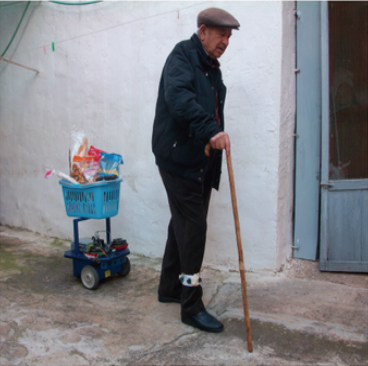
\includegraphics[width=0.45\textwidth]{figs/img/CompaRob}
    %     \caption{CompaRob}
    %     %\label{fig:sysBlockDiag}
    % \end{figure}
\end{frame}

%----------------------------------

% \begin{frame}{Literature Review}
%   \begin{block}{Existing Solution}
%         Gated Recurrent Unit (GRU) network with LiDAR sensor and camera to map the customer~\cite{islam_lam_fukuda_kobayashi_kuno_2019}
%   \end{block}
%     \begin{figure}[b]
%         \centering
%         \includegraphics[width=0.40\textwidth]{figs/img/ShoppingSuportRobot}
%         \caption{Shopping Support Robot}
%         %\label{fig:sysBlockDiag}
%     \end{figure}
% \end{frame}

% %----------------------------------

% \begin{frame}{Literature Review}
%   \begin{block}{Existing Solution}
%     Arduino MEGA 2560, six ultrasonic sensors, two DC motors with Pulse Width Modulation (PWM), an Android Studio IDE device, and Bluetooth~\cite{Rawashdeh2017-Person}
%   \end{block}
%     \begin{figure}[b]
%         \centering
%         \includegraphics[width=0.50\textwidth]{figs/img/SmartCart}
%         \caption{Smart Cart Robot}
%         %\label{fig:sysBlockDiag}
%     \end{figure}
% \end{frame}

%----------------------------------

\begin{frame}{Existing Solutions}
  \begin{block}{Problems}
    \begin{itemize}
      \item Require line-of-sight between robot and user
      \item Some require costly dedicated image processing hardware
    \end{itemize}
  \end{block}
  \pause
  \begin{block}{Benefits of Proposed Solution}
    \begin{itemize}
      \item Line-of-sight is not required since analog RF signals will be used
      \item RF components are cost-effective
    \end{itemize}
  \end{block}
\end{frame}

%----------------------------------

% \begin{frame}{Literature Review}
%   \begin{block}{Multipath Interference}
%     \begin{itemize}
%       \item Proposed solutions to multipath interference
%       \begin{itemize}
%         \item Course estimation calculations such as recieved signal strength indicator (RSSI) and time difference of arrival (TDoA)
%         \item IEEE 802.11b wireless Ethernet device to measure RF signals
%         \item Sampling radio signal strength (RSS) at discrete points without too much deviation from the robot's desired position
%       \end{itemize}
%     \end{itemize}
%   \end{block}
%       \begin{figure}[b]
%         \centering
%         \includegraphics[width=0.40\textwidth]{figs/img/MultipathFading}
%         \caption{Multipath Fading}
%         %\label{fig:sysBlockDiag}
%     \end{figure}
% \end{frame}

% %----------------------------------

% \begin{frame}{Literature Review}
%   \begin{block}{Challenges}
%     \begin{itemize}
%       \item Communication between the robot and the remote
%       \item Buffer distance between the robotic cart and the customer without using line of sight sensing
%     \end{itemize}
%   \end{block}
% \end{frame}

%----------------------------------

\section{System Requirements}
\begin{frame}{System Requirements}
  \begin{block}{Specifications}
    \begin{itemize}
      \item Cart should be able to follow the remote target
      \item Cart should maintain a distance of 1~[\si{\meter}] to 1.5~[\si{\meter}] from the remote target.
      \item Cart should be able to attain a speed of at least 1~[\si{\meter\per\second}]
      \item Cart should not require line-of-sight to follow remote
     \end{itemize}
  \end{block}
\end{frame}

%----------------------------------


%----------------------------------

\section{Concluding Remarks}
\begin{frame}{Concluding Remarks}
  \begin{block}{Project goals}
    \begin{LARGE}
      \begin{itemize}
        \item Develop a robotic cart system utilizing wireless signal strength to locate and follow the user.
        \begin{itemize}
          \item Does not require line-of-sight
          \item Low-cost design
        \end{itemize}
      \end{itemize}
    \end{LARGE}
  \end{block}
  \begin{block}{Anticipated Challenges}
    \begin{itemize}
      \item Inaccurate distance measurements due to multipath effect from environment
      \item Achieving full 360\textdegree measurement in short enough time
    \end{itemize}
  \end{block}
\end{frame}

%----------------------------------

\section{References}

% \begin{frame}{References}
%   \bibliographystyle{IEEEtran}
%   \begin{itemize}
%     \item N. Rawashdeh, R. Haddad, O. Jadallah, and A. To’ma, “A person-following
% robotic cart controlled via a smartphone application: design and evaluation,”
% 09 2017, pp. 1–5.
%     \item M. M. Islam, A. Lam, H. Fukuda, Y. Kobayashi, and Y. Kuno, “An intelligent
% shopping support robot: understanding shopping behavior from 2d skeleton data using gru network,” ROBOMECH Journal, vol. 6, no. 1, 2019.
%     \item J. Sales, J. Marti, R. Marin Prades, E. Cervera, and P. Sanz, “Comparob: The
% shopping cart assistance robot,” International Journal of Distributed Sensor Networks, vol. 2016, pp. 1–15, 02 2016.
%     \item M. S. Miah, J. Knoll, and K. Hevrdejs, “Intelligent range-only mapping and navigation for mobile robots,” IEEE Transactions on Industrial Informatics, vol. 14, no. 3, pp. 1164–1174, 2018.
%     \item D. Li and S. Lane, “A novel and versatile parabolic reflector that significantly
% improves wi-fi reception at different distances and angles,” 2013.
  
%   \end{itemize}


% \end{frame}

%----------------------------------

\begin{frame}{References}

  \bibliographystyle{IEEEtran}
  \bibliography{bib/references.bib}
% 	\begin{itemize}
% 		\item T. Xie, H. Jiang, X. Zhao, and C. Zhang, “A wi-fi-based wireless indoor position sensing system with multipath interference mitigation,” Sep 2019. [Online].
% Available: https://www.ncbi.nlm.nih.gov/pmc/articles/PMC6767237/
% 		\item A. M. Ladd, K. E. Bekris, A. Rudys, L. E. Kavraki, and D. S. Wallach, “Robotics-
% based location sensing using wireless ethernet,” Wireless Networks, vol. 11, no. 1-2, p. 189–204, 2005.
% 		\item M. Lindhe, K. Johansson, and A. Bicchi, “An experimental study of exploiting multipath fading for robot communications,” Robotics: Science and Systems III, 2007.
% 		\item M. Lindhe and K. Johansson, “Using robot mobility to exploit multipath fading,”Wireless Communications, IEEE, vol. 16, pp. 30 – 37, 03 2009.
% 	\end{itemize}

\end{frame}


\end{document}



%%% Local Variables:
%%% mode: latex
%%% TeX-master: t
%%% End:
